\appendix
\chapter{Appendix}
\label{chapter:annex}

% The appendix contains page-sized, non-floating tables and fixed-position
% figure groups. Keep residual space at page bottoms rather than stretching
% paragraph and section spacing around these indivisible blocks.
\raggedbottom

% ══════════════════════════════════════════════════════════════════════════
\section{Selected Hyperparameter Configurations}
\label{appendixA}
% ══════════════════════════════════════════════════════════════════════════

All supervised models were tuned using Optuna with the TPE sampler and MedianPruner: 50 trials with a PR-AUC objective, five-fold stratified cross-validation for the classical models, and one 80/20 holdout within DEV for FT-Transformer. The selected configurations are reported below. One-Class SVM uses the default scikit-learn parameters and is excluded from the Optuna search. The tables report the baseline condition (strategy\,=\,None); the same configurations are reused for all imbalance-strategy experiments.

\par\medskip\noindent\begin{minipage}{\linewidth}\centering
\small
\captionof{table}[Selected hyperparameters on ULB 2013]{Hyperparameter configurations selected by Optuna on ULB 2013 (strategy\,=\,None).}
\label{tab:hyperparams_ulb}
\begin{tabular}{l l r}
\toprule
Model & Hyperparameter & Selected Value \\
\midrule
\multirow{2}{*}{Logistic Regression$^\dagger$}
  & $C$ (inverse regularisation strength) & 0.0783 \\
  & \texttt{l1\_ratio}$^\dagger$ & 0.791 \\
\midrule
\multirow{4}{*}{Random Forest}
  & \texttt{n\_estimators} & 400 \\
  & \texttt{max\_depth} & 30 \\
  & \texttt{min\_samples\_split} & 6 \\
  & \texttt{min\_samples\_leaf} & 2 \\
\midrule
\multirow{8}{*}{LightGBM}
  & \texttt{num\_leaves} & 24 \\
  & \texttt{learning\_rate} & 0.01186 \\
  & \texttt{min\_child\_samples} & 24 \\
  & \texttt{reg\_alpha} & 0.0606 \\
  & \texttt{reg\_lambda} & 3.114 \\
  & \texttt{subsample} & 0.966 \\
  & \texttt{colsample\_bytree} & 0.762 \\
  & \texttt{n\_estimators} & 511 \\
\midrule
\multirow{5}{*}{CatBoost}
  & \texttt{learning\_rate} & 0.01664 \\
  & \texttt{depth} & 10 \\
  & \texttt{l2\_leaf\_reg} & 2.485 \\
  & \texttt{min\_data\_in\_leaf} & 65 \\
  & \texttt{iterations} & 534 \\
\midrule
\multirow{10}{*}{FT-Transformer}
  & \texttt{d\_token} & 256 \\
  & \texttt{n\_blocks} & 2 \\
  & \texttt{attention\_n\_heads} & 8 \\
  & \texttt{attention\_dropout} & 0.209 \\
  & \texttt{ffn\_d\_hidden\_factor} & 2.431 \\
  & \texttt{ffn\_dropout} & 0.157 \\
  & \texttt{residual\_dropout} & 0.168 \\
  & \texttt{learning\_rate} & $1.92 \times 10^{-4}$ \\
  & \texttt{weight\_decay} & $4.30 \times 10^{-4}$ \\
  & \texttt{batch\_size} & 512 \\
\midrule
OCSVM & \multicolumn{2}{l}{Default scikit-learn parameters (no HPO)} \\
\bottomrule
\end{tabular}
\end{minipage}\par\medskip

{\small\noindent $^\dagger$~Logistic Regression was tuned with \texttt{solver=`saga'} and default \texttt{penalty=`l2'}. Optuna suggested \texttt{l1\_ratio} during the search, but this parameter only applies to \texttt{penalty=`elasticnet'} and has no effect here. The effective tuned parameter is $C$ only.}

\par\medskip\noindent\begin{minipage}{\linewidth}\centering
\small
\captionof{table}[Selected hyperparameters on BAF Base]{Hyperparameter configurations selected by Optuna on BAF Base (strategy\,=\,None).}
\label{tab:hyperparams_baf}
\begin{tabular}{l l r}
\toprule
Model & Hyperparameter & Selected Value \\
\midrule
\multirow{2}{*}{Logistic Regression$^\dagger$}
  & $C$ (inverse regularisation strength) & 0.0391 \\
  & \texttt{l1\_ratio}$^\dagger$ & 0.291 \\
\midrule
\multirow{4}{*}{Random Forest}
  & \texttt{n\_estimators} & 500 \\
  & \texttt{max\_depth} & 40 \\
  & \texttt{min\_samples\_split} & 13 \\
  & \texttt{min\_samples\_leaf} & 7 \\
\midrule
\multirow{8}{*}{LightGBM}
  & \texttt{num\_leaves} & 15 \\
  & \texttt{learning\_rate} & 0.01379 \\
  & \texttt{min\_child\_samples} & 18 \\
  & \texttt{reg\_alpha} & 7.077 \\
  & \texttt{reg\_lambda} & $1.39 \times 10^{-5}$ \\
  & \texttt{subsample} & 0.791 \\
  & \texttt{colsample\_bytree} & 0.839 \\
  & \texttt{n\_estimators} & 1696 \\
\midrule
\multirow{5}{*}{CatBoost}
  & \texttt{learning\_rate} & 0.03343 \\
  & \texttt{depth} & 4 \\
  & \texttt{l2\_leaf\_reg} & 7.853 \\
  & \texttt{min\_data\_in\_leaf} & 22 \\
  & \texttt{iterations} & 1394 \\
\midrule
\multirow{10}{*}{FT-Transformer}
  & \texttt{d\_token} & 64 \\
  & \texttt{n\_blocks} & 2 \\
  & \texttt{attention\_n\_heads} & 8 \\
  & \texttt{attention\_dropout} & 0.225 \\
  & \texttt{ffn\_d\_hidden\_factor} & 2.247 \\
  & \texttt{ffn\_dropout} & 0.112 \\
  & \texttt{residual\_dropout} & 0.143 \\
  & \texttt{learning\_rate} & $3.79 \times 10^{-4}$ \\
  & \texttt{weight\_decay} & $1.77 \times 10^{-6}$ \\
  & \texttt{batch\_size} & 512 \\
\midrule
OCSVM & \multicolumn{2}{l}{Default scikit-learn parameters (no HPO)} \\
\bottomrule
\end{tabular}
\end{minipage}\par\medskip

\clearpage

% ══════════════════════════════════════════════════════════════════════════
\section{FT-Transformer Attention Diagnostics --- Individual Case Bar Charts}
\label{appendixB}
% ══════════════════════════════════════════════════════════════════════════

The following figures supplement Section~\ref{sec:attention_diagnostics} (p.~\pageref{sec:attention_diagnostics}) of the Results and Discussion chapter. Each bar chart shows the final-layer, head-averaged per-feature attention weight for one selected test case, with categorical features in orange and numerical features in blue. The dashed horizontal line marks the uniform reference ($1/31 \approx 3.2\%$). All six cases are close to the decision threshold ($\tau = 0.058$), with predicted fraud scores within $0.001$ of that value.

\begin{figure}[H]
\centering
\begin{subfigure}[b]{0.82\textwidth}
  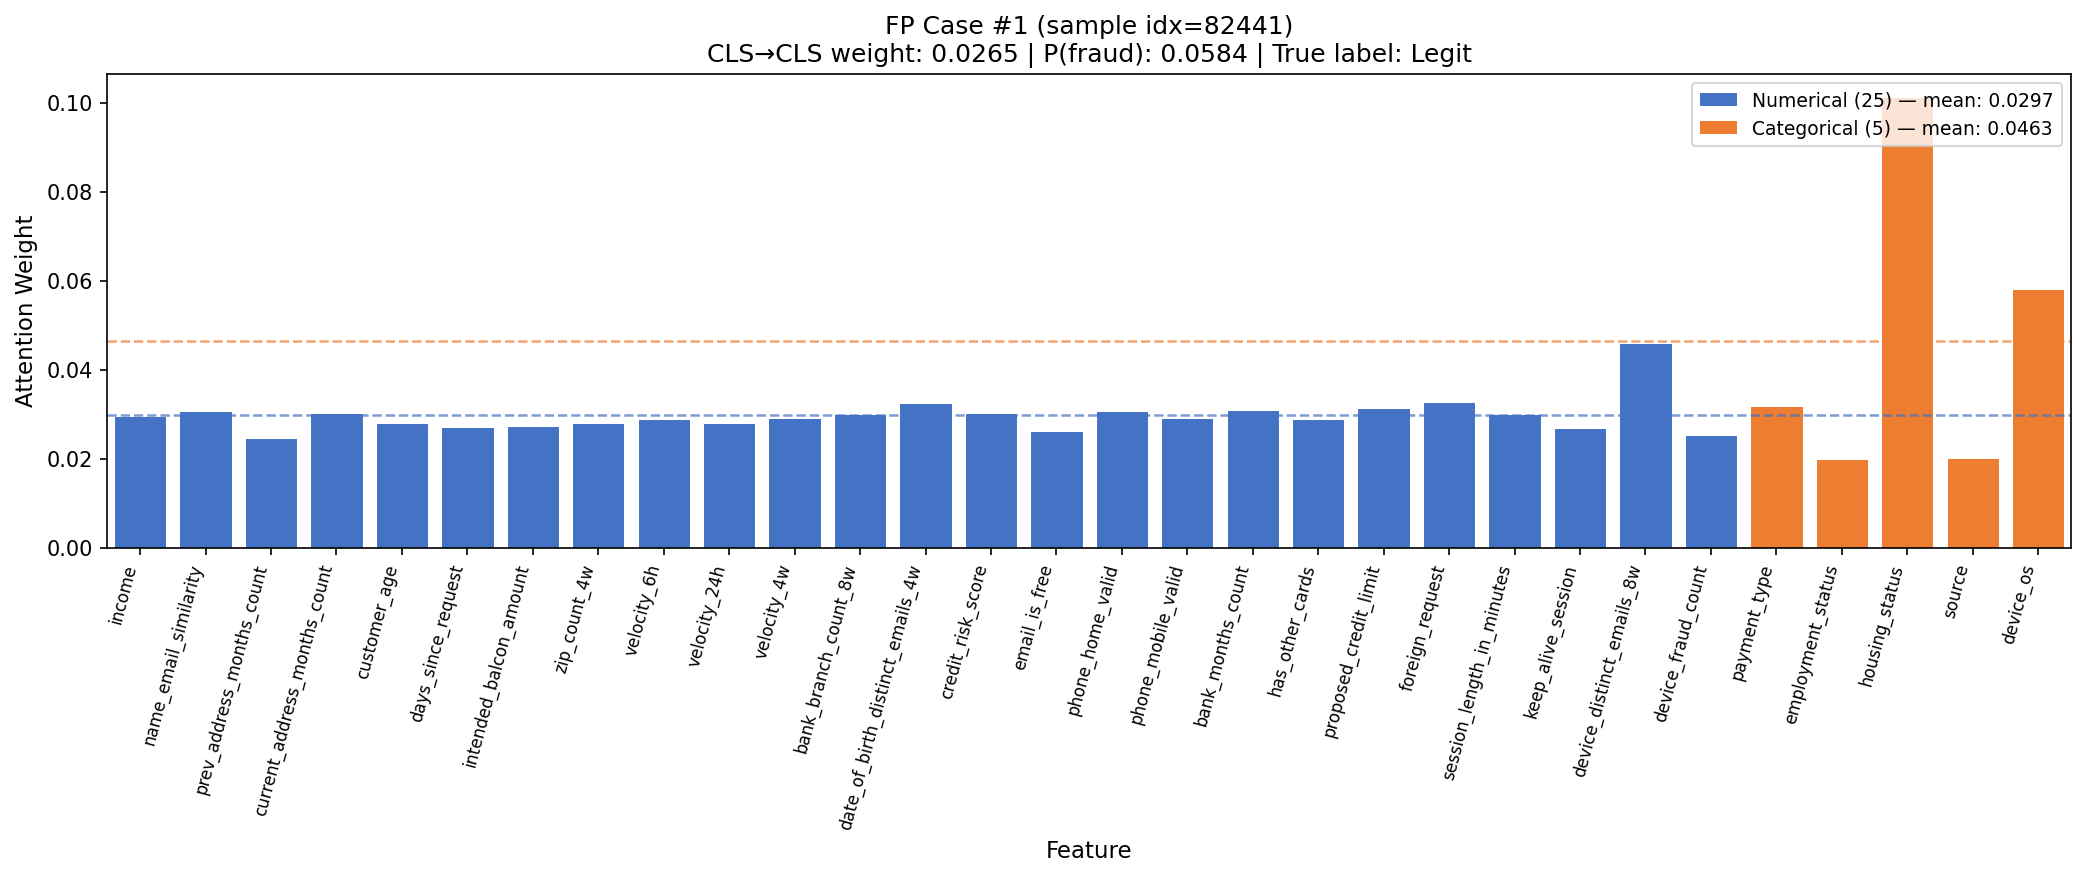
\includegraphics[width=\textwidth]{figures/baf/attention_bar_FP_1.png}
  \caption[FP Case 1]{FP Case 1 (score\,$=\,0.05844$, true label: Legitimate)}
\end{subfigure}

\vspace{0.5em}

\begin{subfigure}[b]{0.82\textwidth}
  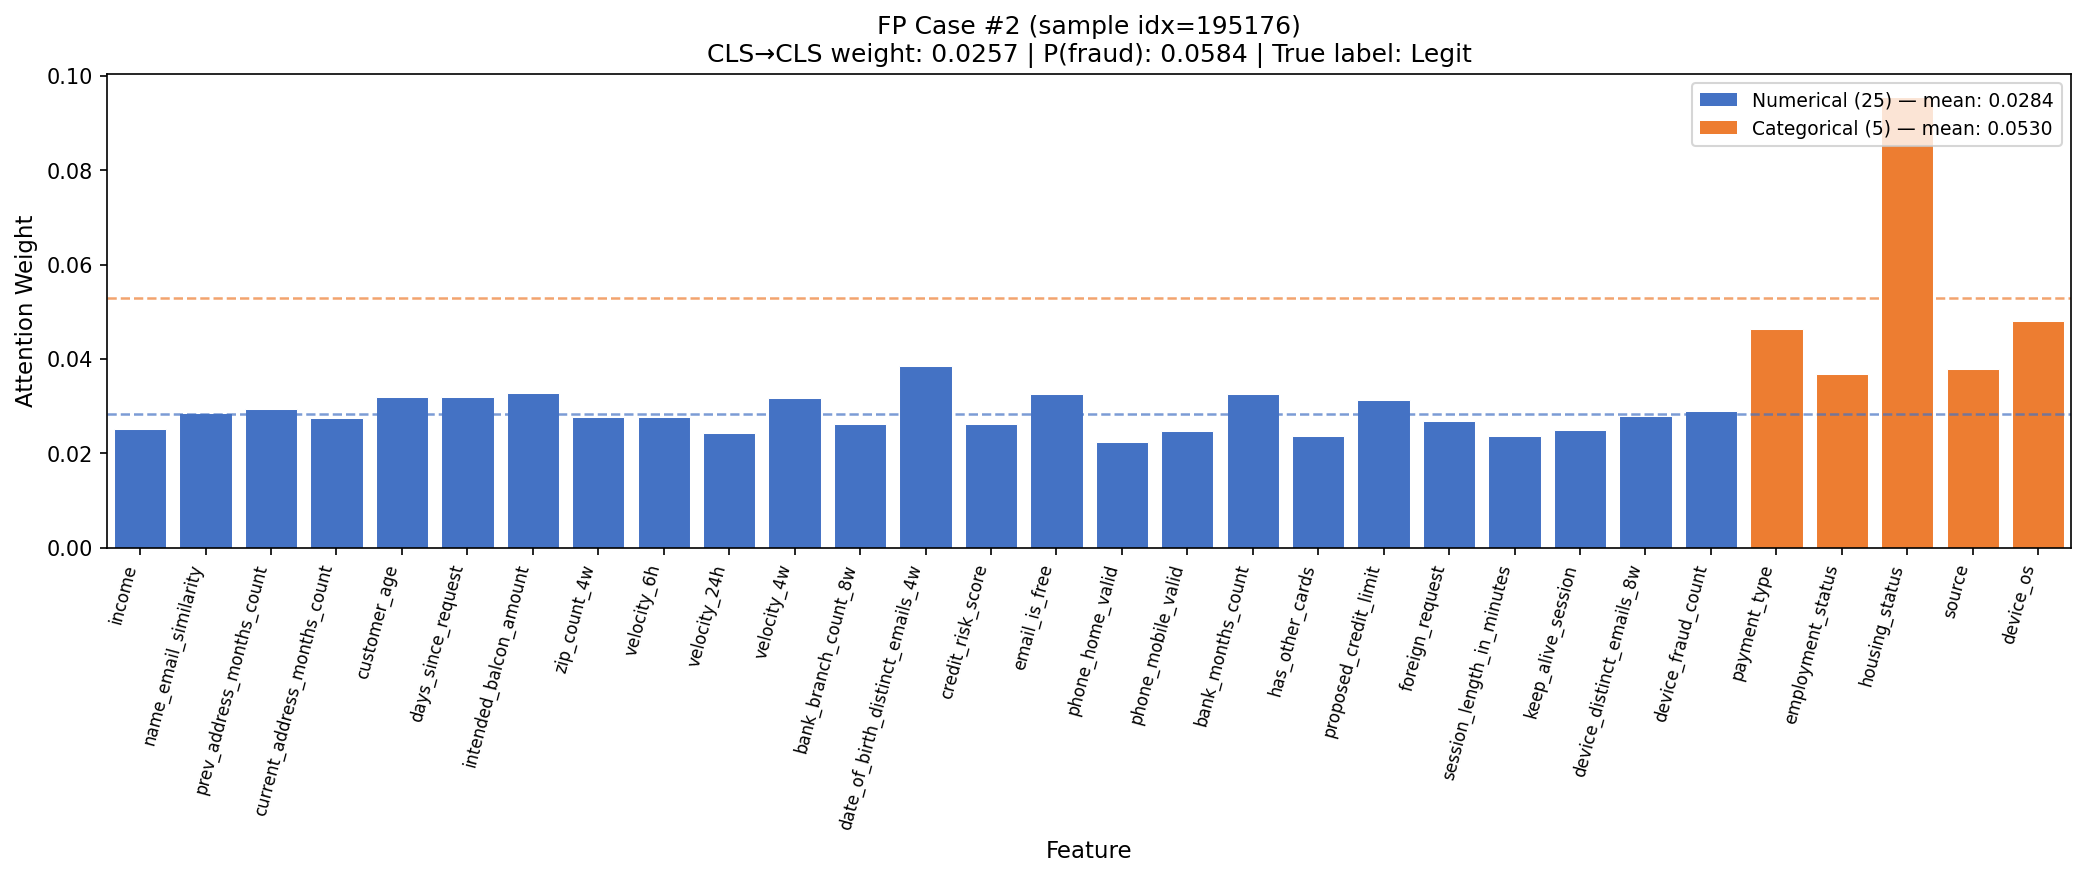
\includegraphics[width=\textwidth]{figures/baf/attention_bar_FP_2.png}
  \caption[FP Case 2]{FP Case 2 (score\,$=\,0.05844$, true label: Legitimate)}
\end{subfigure}

\vspace{0.5em}

\begin{subfigure}[b]{0.82\textwidth}
  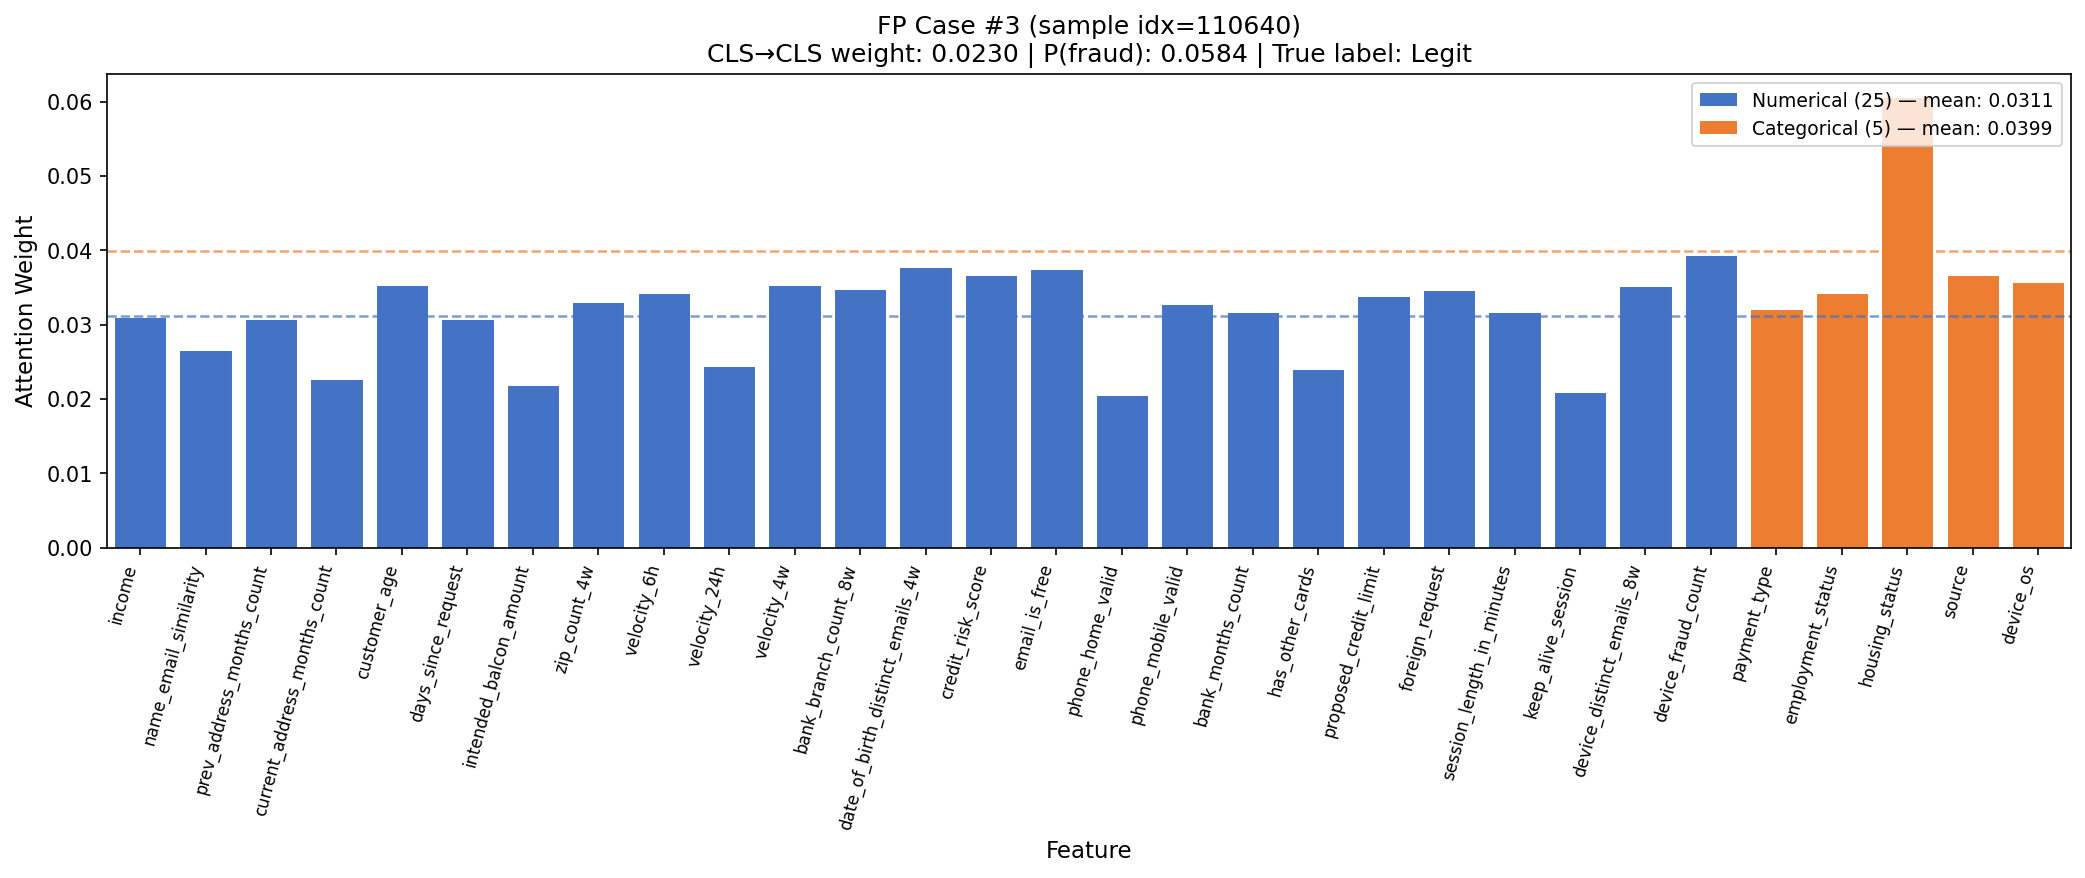
\includegraphics[width=\textwidth]{figures/baf/attention_bar_FP_3.png}
  \caption[FP Case 3]{FP Case 3 (score\,$=\,0.05844$, true label: Legitimate)}
\end{subfigure}

\caption[Per-feature attention for three false-positive cases]{Final-layer, head-averaged per-feature attention weights for three false-positive cases (BAF Base). Orange bars\,=\,categorical features; blue bars\,=\,numerical features. The dashed line indicates the uniform attention reference ($1/31 \approx 3.2\%$). All cases have scores just above $\tau = 0.058$.}
\label{fig:attention_bar_fp}
\end{figure}

\clearpage

\begin{figure}[H]
\centering
\begin{subfigure}[b]{0.82\textwidth}
  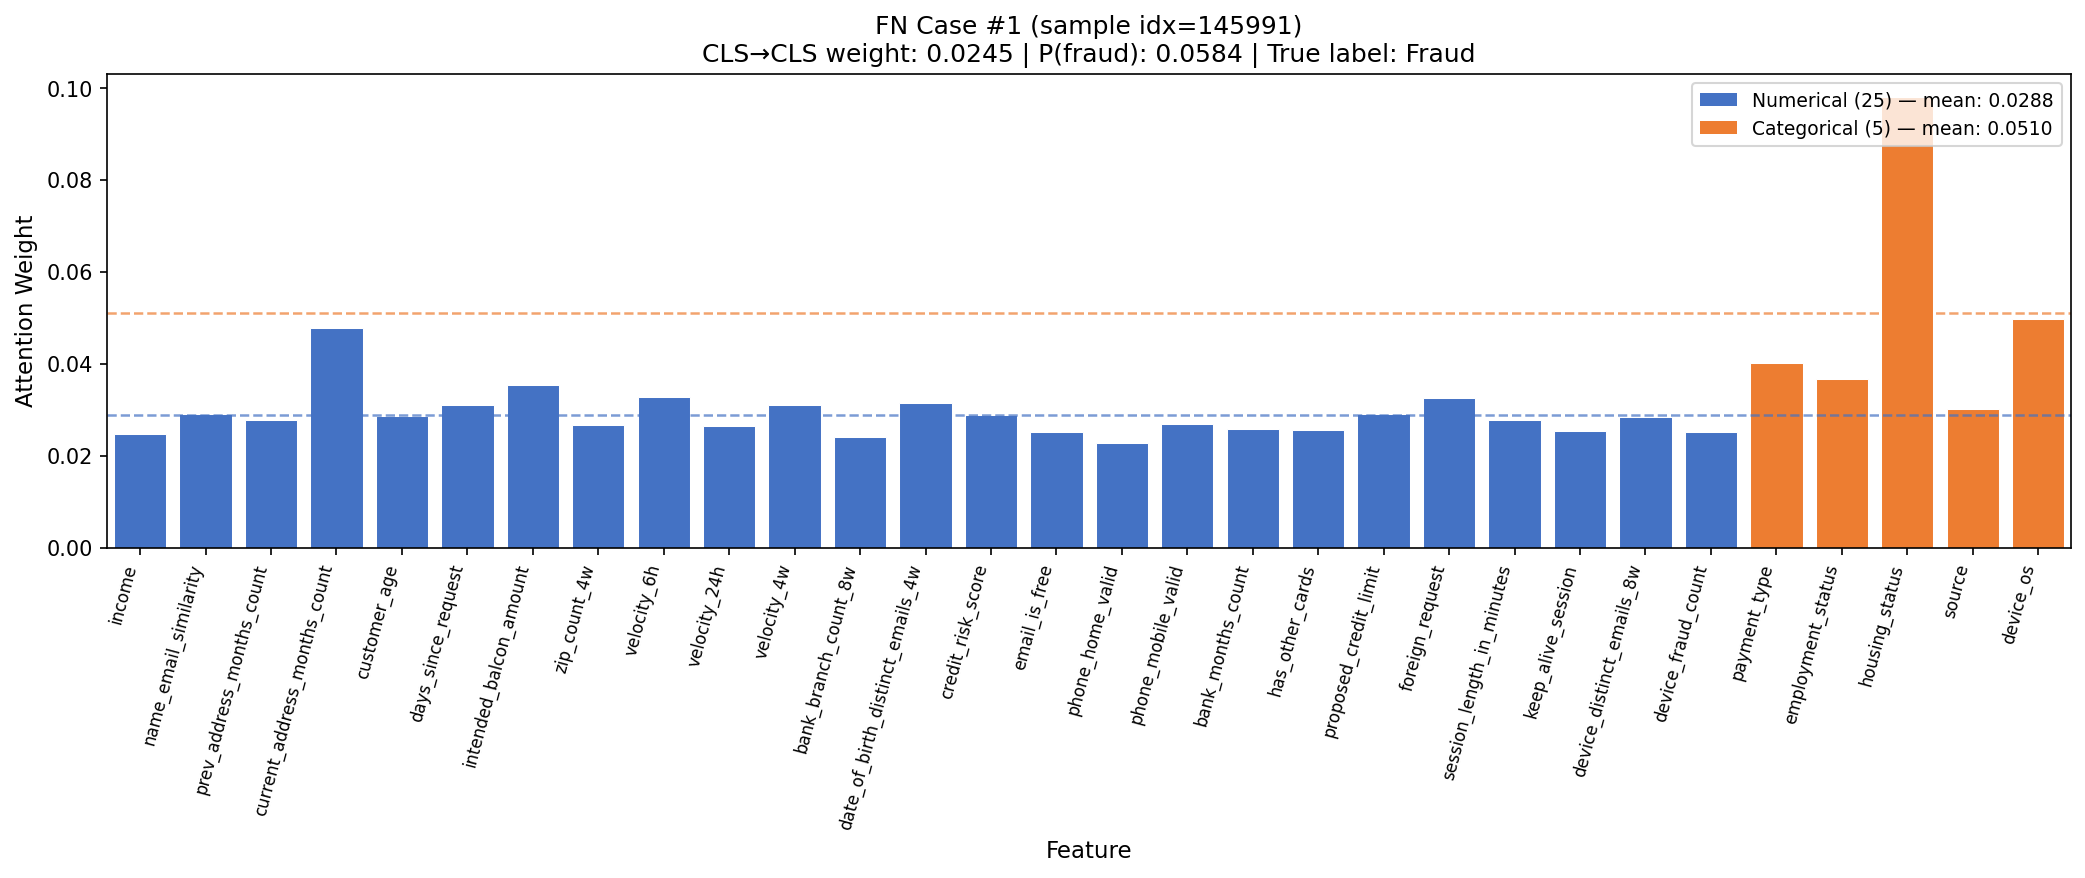
\includegraphics[width=\textwidth]{figures/baf/attention_bar_FN_1.png}
  \caption[FN Case 1]{FN Case 1 (score\,$=\,0.05842$, true label: Fraud)}
\end{subfigure}

\vspace{0.5em}

\begin{subfigure}[b]{0.82\textwidth}
  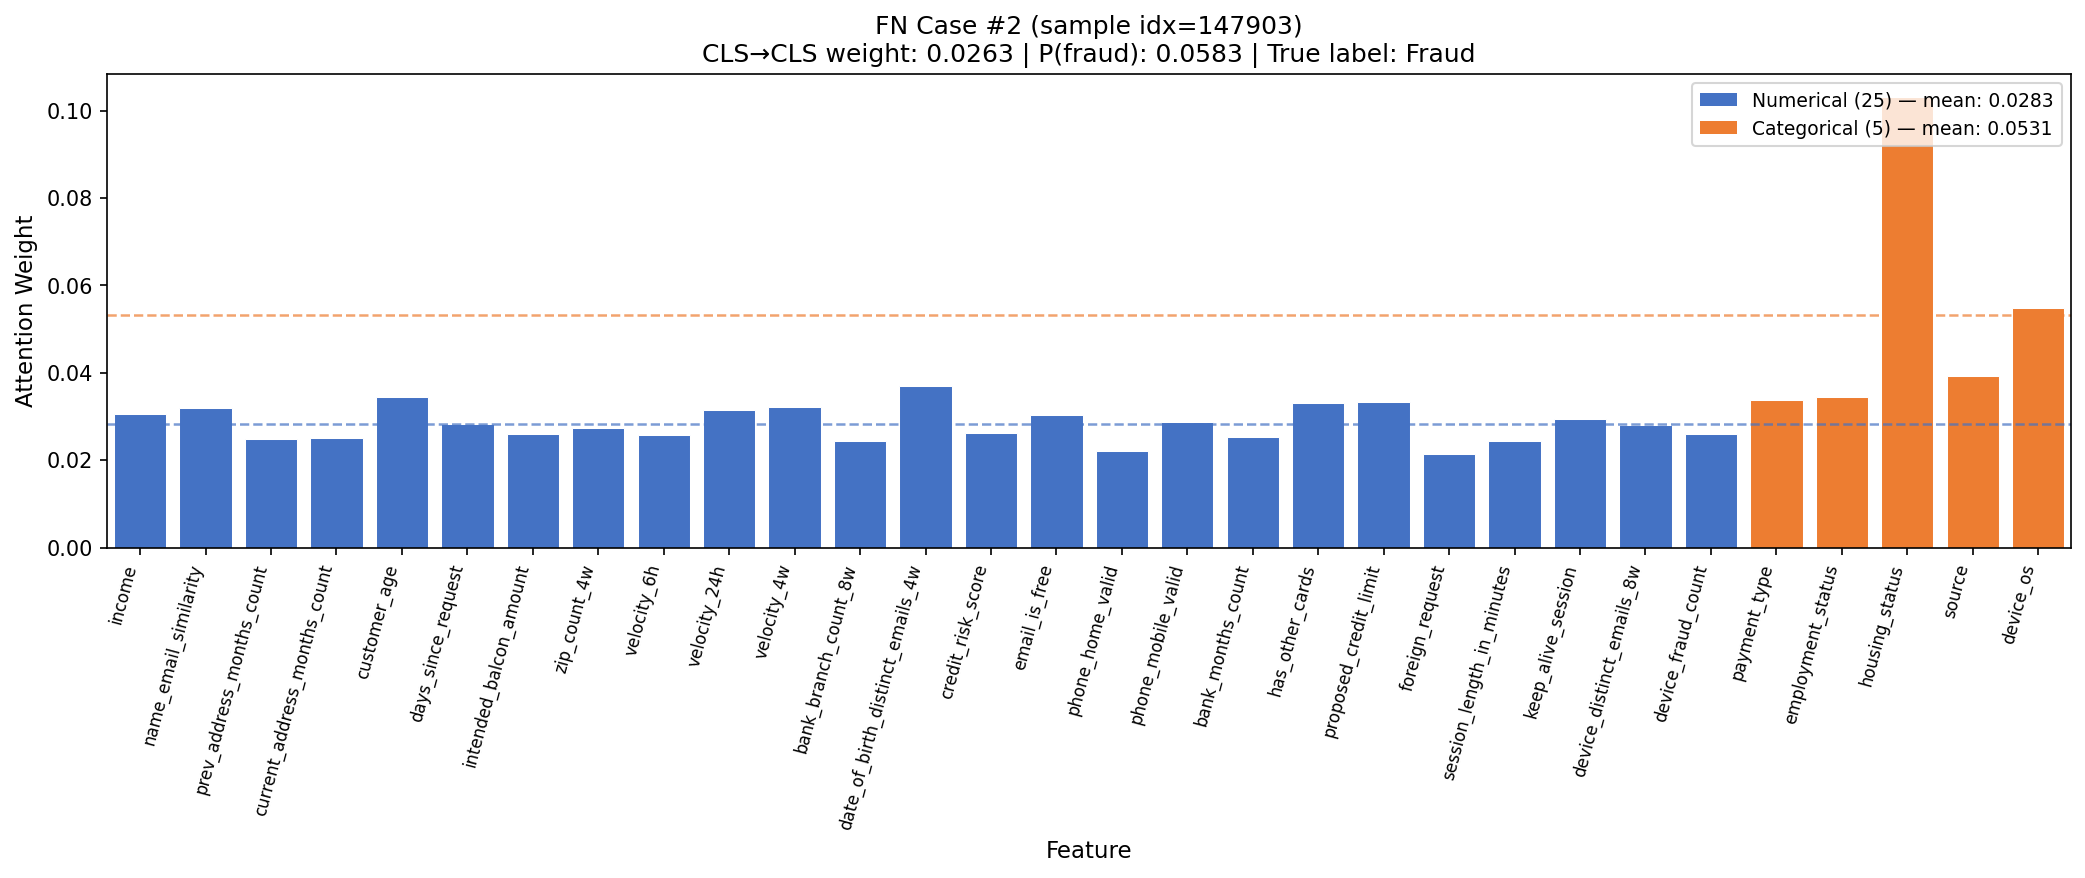
\includegraphics[width=\textwidth]{figures/baf/attention_bar_FN_2.png}
  \caption[FN Case 2]{FN Case 2 (score\,$=\,0.05829$, true label: Fraud)}
\end{subfigure}

\vspace{0.5em}

\begin{subfigure}[b]{0.82\textwidth}
  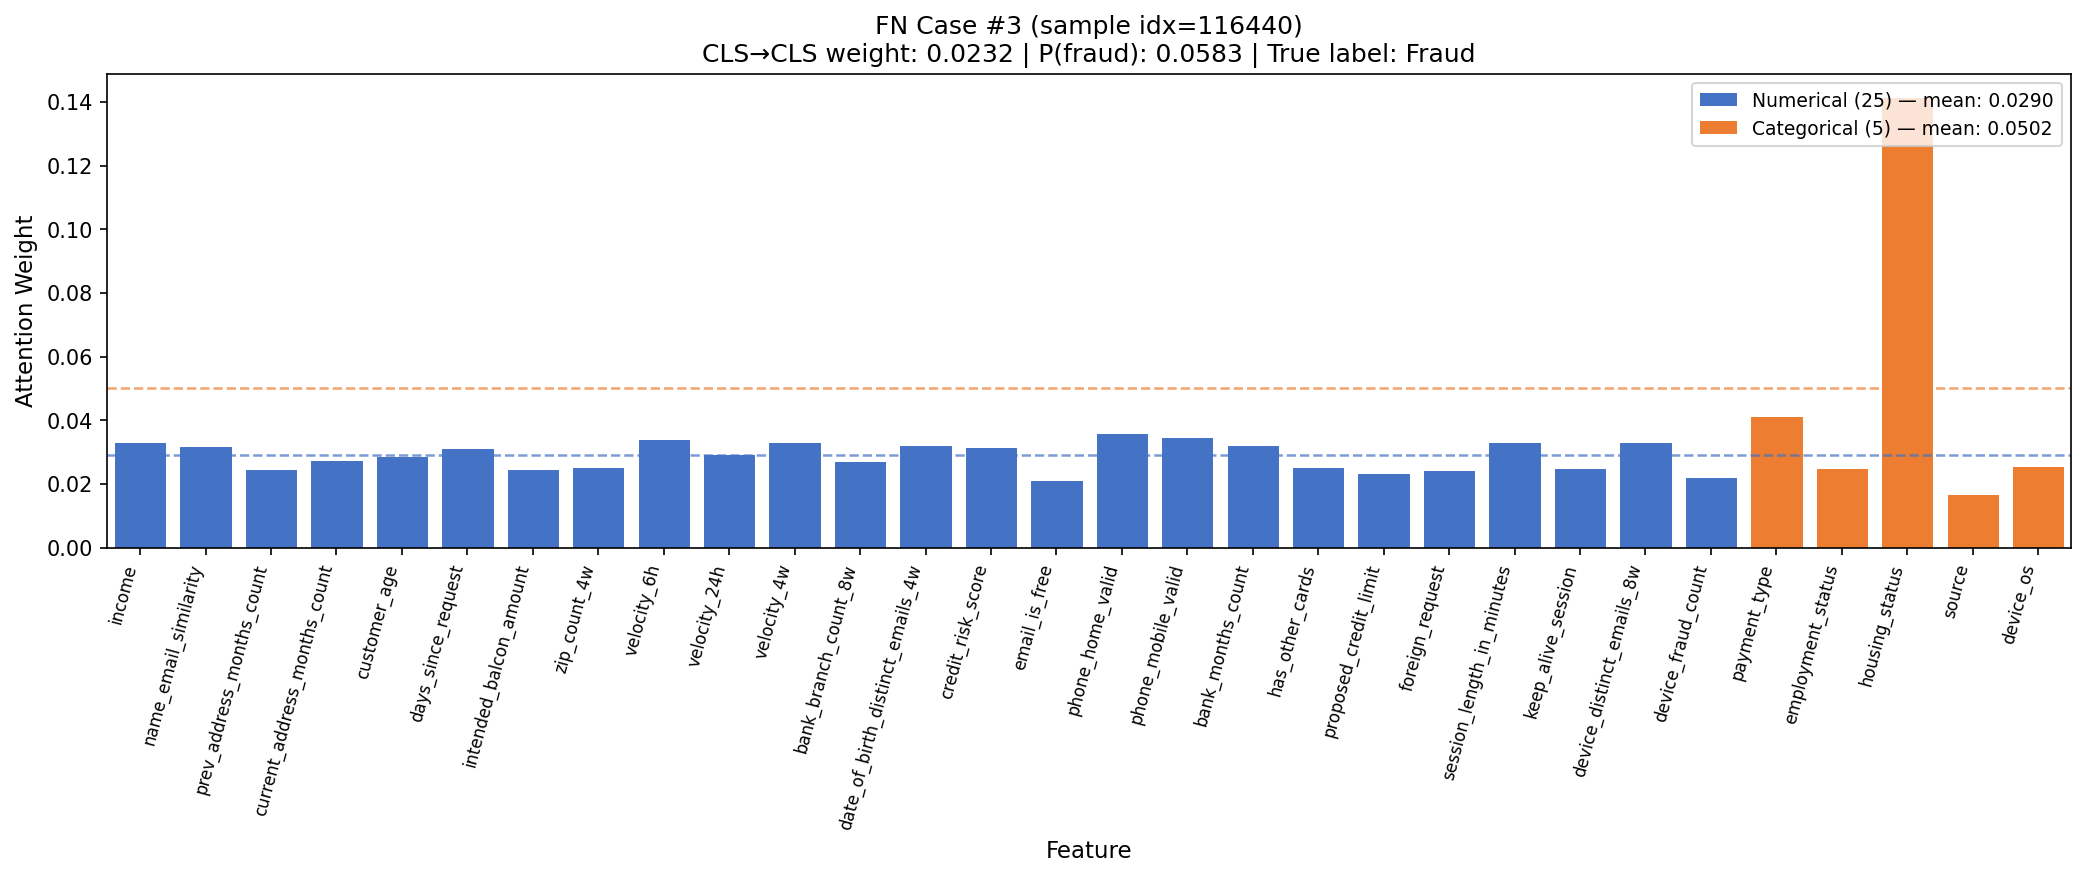
\includegraphics[width=\textwidth]{figures/baf/attention_bar_FN_3.png}
  \caption[FN Case 3]{FN Case 3 (score\,$=\,0.05828$, true label: Fraud)}
\end{subfigure}

\caption[Per-feature attention for three false-negative cases]{Final-layer, head-averaged per-feature attention weights for three false-negative cases (BAF Base). Orange bars\,=\,categorical features; blue bars\,=\,numerical features. The dashed line indicates the uniform attention reference ($1/31 \approx 3.2\%$). All cases have scores just below $\tau = 0.058$. The selected false-positive and false-negative cases show a similar diffuse pattern; this diagnostic does not capture earlier layers or individual attention heads.}
\label{fig:attention_bar_fn}
\end{figure}

Across Figures~\ref{fig:attention_bar_fp} and~\ref{fig:attention_bar_fn}, the selected cases show no strongly dominant feature in the inspected final-layer average. Their similarity to the aggregate view is descriptive only: the figures do not determine whether individual heads or earlier layers contain more concentrated patterns.

% Ship the final Appendix page with natural spacing, then restore the default
% pagination before the bibliography.
\clearpage
\flushbottom
